\let\negmedspace\undefined
\let\negthickspace\undefined
\documentclass[journal]{IEEEtran}
\usepackage[a5paper, margin=10mm, onecolumn]{geometry}
%\usepackage{lmodern} % Ensure lmodern is loaded for pdflatex
\usepackage{tfrupee} % Include tfrupee package

\setlength{\headheight}{1cm} % Set the height of the header box
\setlength{\headsep}{0mm}     % Set the distance between the header box and the top of the text

\usepackage{gvv-book}
\usepackage{gvv}
\usepackage{cite}
\usepackage{amsmath,amssymb,amsfonts,amsthm}
\usepackage{algorithmic}
\usepackage{graphicx}
\usepackage{textcomp}
\usepackage{xcolor}
\usepackage{txfonts}
\usepackage{listings}
\usepackage{enumitem}
\usepackage{mathtools}
\usepackage{gensymb}
\usepackage{comment}
\usepackage[breaklinks=true]{hyperref}
\usepackage{tkz-euclide} 
\usepackage{listings}
% \usepackage{gvv}                                        
\def\inputGnumericTable{}                                 
\usepackage[latin1]{inputenc}                                
\usepackage{color}                                            
\usepackage{array}                                            
\usepackage{longtable}                                       
\usepackage{calc}                                             
\usepackage{multirow}                                         
\usepackage{hhline}                                           
\usepackage{ifthen}                                           
\usepackage{lscape}
\begin{document}

\bibliographystyle{IEEEtran}
\vspace{3cm}

\title{1.4.26}
\author{EE25BTECH11010 - Arsh Dhoke}
{\let\newpage\relax\maketitle}

\renewcommand{\thefigure}{\theenumi}
\renewcommand{\thetable}{\theenumi}
\setlength{\intextsep}{10pt}
\numberwithin{equation}{enumi}
\numberwithin{figure}{enumi}
\renewcommand{\thetable}{\theenumi}

\parindent 0px
\textbf{Question:} \\
The position vector of the point which divides the join of points $2\vec{a} - 3\vec{b}$ and $\vec{a} + \vec{b}$ in the ratio $3:1$ is \underline{\hspace{2cm}}.

\solution \\

\begin{align}
    \vec{P} &= 2\vec{a}-3\vec{b}\\
    \vec{Q} &= \vec{a}+\vec{b}
\end{align}

Now, the matrix form for $\vec{Q}$ and $\vec{P}$ is:
\begin{align}
\myvec{\vec{Q} & \vec{P}}
=\myvec{\vec{a} & \vec{b}}
\myvec{1 & 2 \\ 1 & -3}
\end{align}

Using the section formula, the point $\vec{R}$ dividing $\vec{Q} - \vec{P}$ in ratio $3:1$ is:
\begin{align}
\vec{R} &= \frac{3\vec{Q} + 1\vec{P}}{3+1} \\
\vec{R} &= \frac{1}{4} \cdot \myvec{\vec{Q} & \vec{P}} \myvec{3 \\ 1} \\
\vec{R} &= \frac{1}{4} \cdot \myvec{\vec{a} & \vec{b}}\myvec{1 & 2 \\ 1 & -3} \myvec{3 \\ 1} \\
\vec{R} &= \frac{1}{4} \cdot \myvec{\vec{a} & \vec{b}} \myvec{5 \\ 0} \\
\vec{R} &= \frac{1}{4} \cdot \myvec{5\vec{a}}  
\end{align}




\begin{figure}[ht!]
\centering
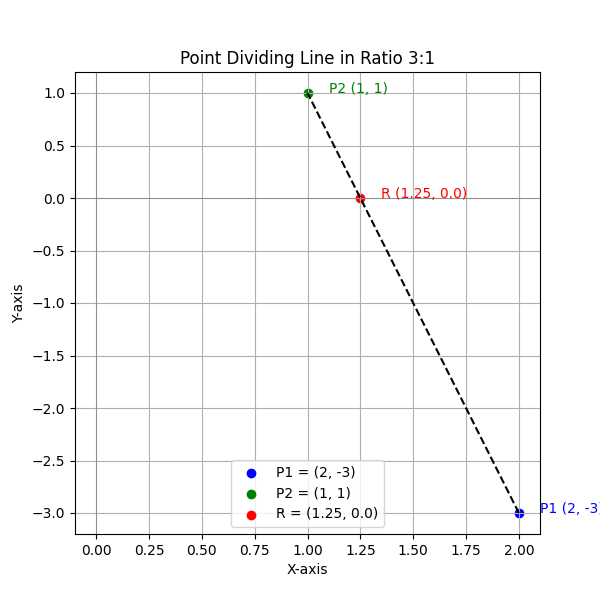
\includegraphics[height=0.5\textheight, keepaspectratio]{figs/q1.png}
\caption{Graph for question 1}
\end{figure}

\end{document}
